

\tikzset{every picture/.style={line width=0.75pt}} %set default line width to 0.75pt        

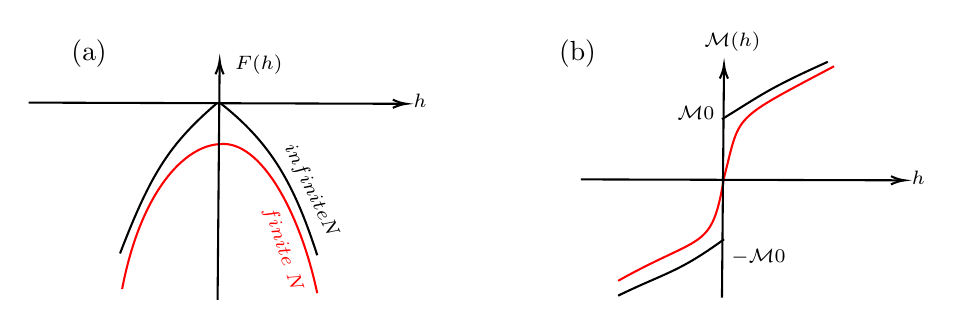
\begin{tikzpicture}[x=0.75pt,y=0.75pt,yscale=-1,xscale=1]
%uncomment if require: \path (0,170); %set diagram left start at 0, and has height of 170

%Straight Lines [id:da23635493997133195] 
\draw    (59,49) -- (239,49.58) ;
\draw [shift={(241,49.58)}, rotate = 180.18] [color={rgb, 255:red, 0; green, 0; blue, 0 }  ][line width=0.75]    (6.56,-1.97) .. controls (4.17,-0.84) and (1.99,-0.18) .. (0,0) .. controls (1.99,0.18) and (4.17,0.84) .. (6.56,1.97)   ;
%Curve Lines [id:da18235450228974837] 
\draw    (151,49) .. controls (176,68.52) and (187,88.52) .. (198,122.52) ;
%Curve Lines [id:da1225976391320428] 
\draw    (150,49) .. controls (127,68.8) and (118,82.67) .. (103,121.67) ;
%Curve Lines [id:da22793112325804687] 
\draw [color={rgb, 255:red, 255; green, 0; blue, 0 }  ,draw opacity=1 ]   (151,69) .. controls (171,66.8) and (190,102.8) .. (198,140.8) ;
%Curve Lines [id:da9488433252498562] 
\draw [color={rgb, 255:red, 255; green, 0; blue, 0 }  ,draw opacity=1 ]   (151,69) .. controls (134,69.8) and (113,91.8) .. (104,138.8) ;
%Straight Lines [id:da1517918266482663] 
\draw    (150,144) -- (150.98,30.8) ;
\draw [shift={(151,28.8)}, rotate = 90.5] [color={rgb, 255:red, 0; green, 0; blue, 0 }  ][line width=0.75]    (6.56,-1.97) .. controls (4.17,-0.84) and (1.99,-0.18) .. (0,0) .. controls (1.99,0.18) and (4.17,0.84) .. (6.56,1.97)   ;
%Curve Lines [id:da2541371388654118] 
\draw [color={rgb, 255:red, 255; green, 0; blue, 0 }  ,draw opacity=1 ]   (394,85.2) .. controls (402,54) and (397,58) .. (447,31.5) ;
%Curve Lines [id:da026300410741942226] 
\draw [color={rgb, 255:red, 255; green, 0; blue, 0 }  ,draw opacity=1 ]   (343,134.85) .. controls (384,111.85) and (388,120.85) .. (394,85.2) ;
%Curve Lines [id:da30742639571825414] 
\draw    (393,57) .. controls (412,45.35) and (415,42.35) .. (444,29.35) ;
%Curve Lines [id:da21107772902168997] 
\draw    (343,142) .. controls (366,130.85) and (372,130.85) .. (394,114.85) ;
%Straight Lines [id:da4537306814275738] 
\draw    (393,143) -- (393.98,32.85) ;
\draw [shift={(394,30.85)}, rotate = 90.51] [color={rgb, 255:red, 0; green, 0; blue, 0 }  ][line width=0.75]    (6.56,-1.97) .. controls (4.17,-0.84) and (1.99,-0.18) .. (0,0) .. controls (1.99,0.18) and (4.17,0.84) .. (6.56,1.97)   ;
%Straight Lines [id:da838604604323268] 
\draw    (325,86) -- (479,86.44) ;
\draw [shift={(481,86.45)}, rotate = 180.17] [color={rgb, 255:red, 0; green, 0; blue, 0 }  ][line width=0.75]    (6.56,-1.97) .. controls (4.17,-0.84) and (1.99,-0.18) .. (0,0) .. controls (1.99,0.18) and (4.17,0.84) .. (6.56,1.97)   ;

% Text Node
\draw (157,24.4) node [anchor=north west][inner sep=0.75pt]  [font=\scriptsize]  {$F( h)$};
% Text Node
\draw (243,43.4) node [anchor=north west][inner sep=0.75pt]  [font=\scriptsize]  {$h$};
% Text Node
\draw (179.57,96.47) node [anchor=north west][inner sep=0.75pt]  [font=\scriptsize,color={rgb, 255:red, 255; green, 0; blue, 0 }  ,opacity=1 ,rotate=-71.4]  {$\text{finite} \ N$};
% Text Node
\draw (188.7,65.63) node [anchor=north west][inner sep=0.75pt]  [font=\scriptsize,color={rgb, 255:red, 0; green, 0; blue, 0 }  ,opacity=1 ,rotate=-64.07]  {$\text{infinite } N$};
% Text Node
\draw (483,80.4) node [anchor=north west][inner sep=0.75pt]  [font=\scriptsize]  {$h$};
% Text Node
\draw (383,13.4) node [anchor=north west][inner sep=0.75pt]  [font=\scriptsize]  {$\mathcal{M}( h)$};
% Text Node
\draw (370,49.4) node [anchor=north west][inner sep=0.75pt]  [font=\scriptsize]  {$\mathcal{M}\tund{0}$};
% Text Node
\draw (396,118.25) node [anchor=north west][inner sep=0.75pt]  [font=\scriptsize]  {$-\mathcal{M}\tund{0}$};
% Text Node
\draw (78,17) node [anchor=north west][inner sep=0.75pt]   [align=left] {(a)};
% Text Node
\draw (313,17) node [anchor=north west][inner sep=0.75pt]   [align=left] {(b)};


\end{tikzpicture}
